\section{Método}
\label{sec:metodo}
Al igual que los atributos, los métodos, son componentes dentro del diagrama de
clases que ayudan a la manipulación de los datos, estos brindan el
comportamiento que es propio al objeto.

Director, está dotado de la capacidad para tratar los casos triviales del
manejo de los datos dentro de un objeto, estos casos triviales corresponden a
situaciones en las cuales una de las necesidades de comportammiento para un
objeto viene dado por la urgencia de agregar algún mecanismo que permita
acceder a los atributos del mismo, las acciones comunes de acceso a estos
atributos son las siguientes: definir el valor de un atributo y obtener el
valor de ese atributo, las cuales son solucionadas con los \texttt{setters}
y los \texttt{getters}.

Director, no requiere que se definan explicitamente estos métodos, éste los
genera de manera automática.

Teniendo en cuenta el ejemplo mencionado en la \texttt{Seccion
\ref{sec:atributo}}, Director automáticamente generaría los siguientes métodos
para el lenguaje Java:

\begin{lstlisting}[language=Java, basicstyle=\footnotesize\ttfamily,
label=lst:drt_java_metodo, caption={Java - Generación \texttt{Fragmento \ref{sec:atributo}}}]
  ...
	public String get_nombre(){
		return this.nombre;
		}

	public void set_nombre(String nombre){
		this.nombre = nombre;
		}

	public String get_apellido(){
		return this.apellido;
		}

	public void set_apellido(String apellido){
		this.apellido = apellido;
		}

	public String get_DNI(){
		return this.DNI;
		}
	...
\end{lstlisting}

De todos modos, es posible indicar otros métodos que se deseen incluir en el
modelo. Si se agrega algún $metodo\_generico$ al ejemplo con el que se viene
trabajando, la lista de atributos y modelos quedaría definida de la siguiente
manera.

\begin{lstlisting}[caption={Director - Declaración de Método}, label=lst:drt_java_modelo_metodo_generico]
	private nombre:string
	private apellido:string
	private DNI:string
	public metodo_generico():void
\end{lstlisting}

Lo que resultaría en la generación del ``esqueleto'' necesario para la
implementación de dicho método. Tomando como base lo que ya se hizo en
el \texttt{Fragmento \ref{lst:drt_java_metodo}}, se le agregaría:

\begin{lstlisting}[caption={Java - Generación metodo\_generico agregado en
\texttt{Fragmento \ref{lst:drt_java_modelo_metodo_generico}}}, language=Java, basicstyle=\footnotesize\ttfamily]
  public void metodo_generico() {
		// Implementacion del metodo
		}
\end{lstlisting}

La definición formal del funcionamiento del componente se va a separar en la
parte Léxica y la parte Sintáctica.

\subsubsection{Analizador Léxico}

Iniciando con este componente se puede definir los patrones que rigen su
funcionamiento, esto a través de expresiones regulares.

En primera instancia, para mantenerlo simple, se procede a definir una
expresión regular para un método sin ningun parametro, el resultado se puede
ver en el \texttt{Fragmento \ref{lst:remetnoparam}}.

\begin{lstinputlisting}[basicstyle=\footnotesize\ttfamily, caption={Regex - Método
(sin parámetro(s))},
label=lst:remetnoparam, language=Java]{regex/metodo/metodo_sin_parametros.txt}

complicándolo un poco mas se le adhieren los posibles argumentos que puede
recibir el método, esto se refleja en \texttt{Fragmento
\ref{lst:remetparam}}

\begin{lstinputlisting}[basicstyle=\footnotesize\ttfamily, caption={Regex - Método
  (con parámetro(s))},
  label=lst:remetparam, language=Java]{regex/metodo/metodo_con_parametros.txt}

A continuación se describen los autómatas finitos para la definición de un método y
además se propone separar la definición del mismo en partes para hacer mas
manejable el gráfico, por ejemplo, aquí se separa la definicion de \texttt{parametro}.

\begin{figure}[H]
	\centering
	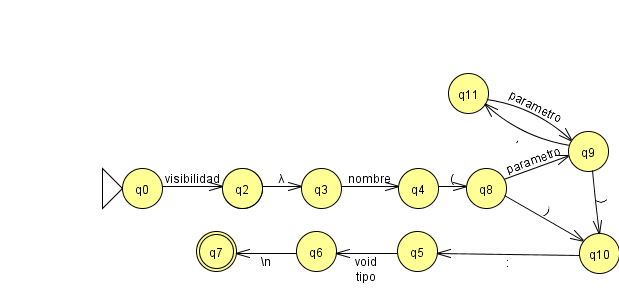
\includegraphics[width=.7\linewidth]{automatas_finitos/metodoDrt.png}
	\caption{Autómata finito - Método}
	\label{fig:metodo_af}
\end{figure}

\begin{figure}[H]
	\centering
	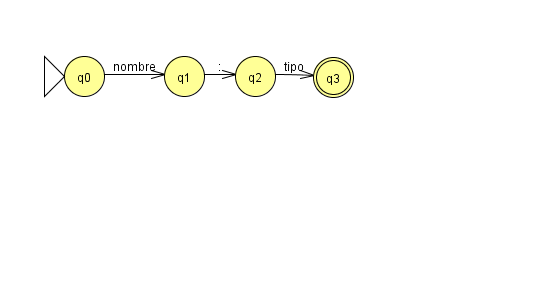
\includegraphics[width=.7\linewidth]{automatas_finitos/parametroDrt.png}
	\caption{Autómata finito - Parámetro}
	\label{fig:metodo_parametro_af}
\end{figure}

\subsubsection{Analizador Sintáctico}

\begin{lstlisting}[caption={BNF - Método}, basicstyle=\footnotesize\ttfamily]
  <metodo>::=<visibilidad><nombre>"("<parametro>")" ":"<tipo>
  <metodo>::=<visibilidad><nombre>"("<parametros>")" ":"<tipo>
\end{lstlisting}

En donde se puede decir que \texttt{parametro(s)} se define de la siguiente
manera:

\begin{lstlisting}[basicstyle=\footnotesize\ttfamily]
  <parametro> ::= <nombre> ":" <tipo>
\end{lstlisting}

\begin{lstlisting}[basicstyle=\footnotesize\ttfamily]
  <parametros> ::= <parametro> | <parametros>
\end{lstlisting}

\subsubsection{Derivaciones Método}

Habiendo definido los patrones y las representaciones visuales que gobiernan
el uso del componente se procede a estudiar los pasos a seguir en cuanto al
análisis sintáctico, aquí se veran las derivaciones que siguen de un ejemplo,
junto con el árbol sintáctico del mismo.

El ejemplo a tomarse para el análisis se describe a continuación:

\begin{lstlisting}
  EJEMPLO: public factorial(n:integer):long \n
\end{lstlisting}

Por cuestiones de espacio y de lo extenso de las derivaciones para los
componentes, se tomaron abreviaciones para los componentes, a continuación
se detalla el significado de cada una de ellos.

\begin{itemize}
  \item \textbf{V}: visibilidad
  \item \textbf{N}: nombre
  \item \textbf{SE}: simbolo especial
  \item \textbf{T}: tipo
  \item \textbf{P}: parametros
\end{itemize}

\begin{lstlisting}[basicstyle=\footnotesize\ttfamily, caption={Derivaciones -
Método}, label=dermet]
  comp-drt -> metodo
  metodo -> V N SE    P   SE SE T SE
  metodo -> V N SE N SE T SE SE T SE
  metodo -> public factorial SE N SE T SE SE T SE
  metodo -> public factorial ( N SE T SE SE T SE
  metodo -> public factorial(n SE T SE SE T SE
  metodo -> public factorial(n: T SE SE T SE
  metodo -> public factorial(n:integer SE SE T SE
  metodo -> public factorial(n:integer) SE T SE
  metodo -> public factorial(n:integer): T SE
  metodo -> public factorial(n:integer):long SE
  metodo -> public factorial(n:integer):long \n
\end{lstlisting}

El árbol sintácico para el ejemplo propuesto y resultante de la derivación de
la gramática libre de contexto se presenta a continuación:

\begin{figure}[H]
  \centering
  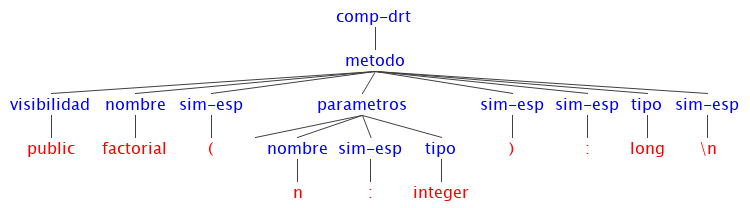
\includegraphics[width=.7\linewidth]{arboles_sintaxis/3_metodo.png}
  \caption{Árbol Sintáctico - Método}
  \label{asmet}
\end{figure}
